% -----------------------------------------------------------------------------
% The MIT License (MIT)
%
% Copyright (c) 2015 Pejman Ghorbanzade
%
% Permission is hereby granted, free of charge, to any person obtaining a copy
% of this software and associated documentation files (the "Software"), to deal
% in the Software without restriction, including without limitation the rights
% to use, copy, modify, merge, publish, distribute, sublicense, and/or sell
% copies of the Software, and to permit persons to whom the Software is
% furnished to do so, subject to the following conditions:
%
% The above copyright notice and this permission notice shall be included in
% all copies or substantial portions of the Software.
%
% THE SOFTWARE IS PROVIDED "AS IS", WITHOUT WARRANTY OF ANY KIND, EXPRESS OR
% IMPLIED, INCLUDING BUT NOT LIMITED TO THE WARRANTIES OF MERCHANTABILITY,
% FITNESS FOR A PARTICULAR PURPOSE AND NONINFRINGEMENT. IN NO EVENT SHALL THE
% AUTHORS OR COPYRIGHT HOLDERS BE LIABLE FOR ANY CLAIM, DAMAGES OR OTHER
% LIABILITY, WHETHER IN AN ACTION OF CONTRACT, TORT OR OTHERWISE, ARISING FROM,
% OUT OF OR IN CONNECTION WITH THE SOFTWARE OR THE USE OR OTHER DEALINGS IN
% THE SOFTWARE.
% -----------------------------------------------------------------------------

\def \topDirectory {../..}

\documentclass[10pt, compress]{beamer}

\usepackage{\topDirectory/template/style/directives}
% -----------------------------------------------------------------------------
% The MIT License (MIT)
%
% Copyright (c) 2015 Pejman Ghorbanzade
%
% Permission is hereby granted, free of charge, to any person obtaining a copy
% of this software and associated documentation files (the "Software"), to deal
% in the Software without restriction, including without limitation the rights
% to use, copy, modify, merge, publish, distribute, sublicense, and/or sell
% copies of the Software, and to permit persons to whom the Software is
% furnished to do so, subject to the following conditions:
%
% The above copyright notice and this permission notice shall be included in
% all copies or substantial portions of the Software.
%
% THE SOFTWARE IS PROVIDED "AS IS", WITHOUT WARRANTY OF ANY KIND, EXPRESS OR
% IMPLIED, INCLUDING BUT NOT LIMITED TO THE WARRANTIES OF MERCHANTABILITY,
% FITNESS FOR A PARTICULAR PURPOSE AND NONINFRINGEMENT. IN NO EVENT SHALL THE
% AUTHORS OR COPYRIGHT HOLDERS BE LIABLE FOR ANY CLAIM, DAMAGES OR OTHER
% LIABILITY, WHETHER IN AN ACTION OF CONTRACT, TORT OR OTHERWISE, ARISING FROM,
% OUT OF OR IN CONNECTION WITH THE SOFTWARE OR THE USE OR OTHER DEALINGS IN
% THE SOFTWARE.
% -----------------------------------------------------------------------------

\course{id}{CS114}
\course{name}{Introduction to Java}
\course{venue}{Mon/Wed, 5:30 PM - 6:45 PM}
\course{semester}{Fall 2015}
\course{department}{Department of Computer Science}
\course{university}{University of Massachusetts Boston}

\instructor{name}{Pejman Ghorbanzade}
\instructor{title}{}
\instructor{position}{Student Instructor}
\instructor{email}{pejman@cs.umb.edu}
\instructor{phone}{617-287-6419}
\instructor{office}{S-3-124B}
\instructor{office-hours}{Mon/Wed 16:00-17:30}
\instructor{address}{University of Massachusetts Boston, 100 Morrissey Blvd., Boston, MA}

\usepackage{\topDirectory/template/style/beamerthemeUmassLecture}
\doc{number}{12}
%\setbeamertemplate{footline}[text line]{}

\begin{document}
\prepareCover

\section{Course Administration}

\begin{slide}
	\begin{block}{Overview}
		\begin{itemize}
			\item[] Object-Oriented Programming
			\item[] Objects
			\item[] Classes
		\end{itemize}
	\end{block}
\end{slide}

\section{Object-Oriented Programming}

\begin{slide}
	\begin{block}{Meet the Daltons!}
		\begin{figure}[H]\centering
			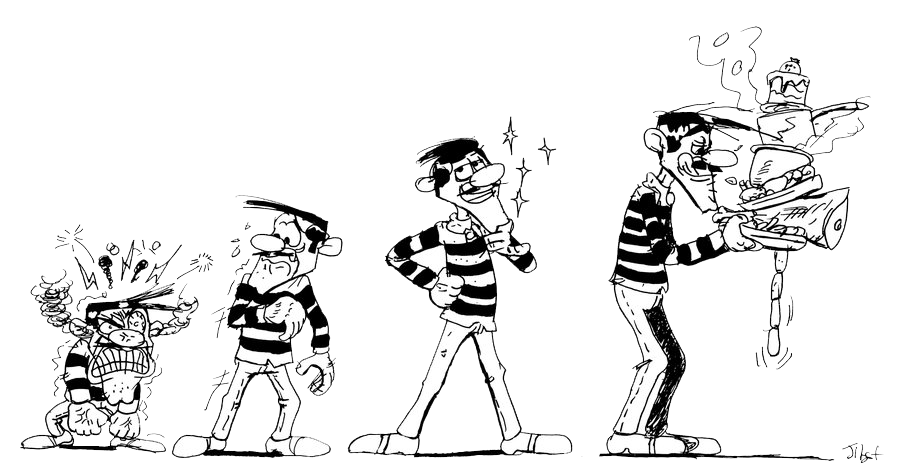
\includegraphics[width=\textwidth]{\topDirectory/template/images/daltons.png}
		\end{figure}
	\end{block}
\end{slide}

\begin{slide}
	\begin{block}{Objective}
		Write a program \texttt{DaltonBrothers.java} that takes height of the four brothers, Joe, William, Jack and Averell.
		The program should output names of the brothers in ascending order of their heights.
	\end{block}
\end{slide}

\begin{slide}
	\begin{block}{Strategy}
		\begin{itemize}
			\item[] Initialize names of brothers in array of Strings
			\item[] Ask heights of brothers and store in array of Double
			\item[] Sort heights of brothers and store new indices
			\item[] Display names of brothers according to new indices
		\end{itemize}
	\end{block}
\end{slide}

\begin{slide}
	\begin{block}{\texttt{DaltonBrothers.java} (v1.0) (Part 1)}
		\begin{minted}[fontsize=\small,tabsize=8, linenos, firstnumber=1]{java}
			import java.util.Scanner;
			public class DaltonBrothers {
			public static void main(String[] args) {
			    String[] names = {"Joe", "William", "Jack", "Averell"};
			    double[] heights = promptHeights(names);
			    int[] indices = sortHeights(heights);
			    printNames(names, indices);
			}
		\end{minted}
	\end{block}
\end{slide}

\begin{slide}
	\begin{block}{\texttt{DaltonBrothers.java} (v1.0) (Part 2)}
		\begin{minted}[fontsize=\small,tabsize=8, linenos, firstnumber=1]{java}
			public static double[] promptHeights(String[] names) {
			    Scanner input = new Scanner(System.in);
			    double[] heights = new double[names.length];
			    for (int i = 0; i < names.length; i++) {
			        System.out.printf("Enter height of %s: ", names[i]);
			        heights[i] = input.nextDouble();
			    }
			    return heights;
			}
		\end{minted}
	\end{block}
\end{slide}

\begin{slide}
	\begin{block}{\texttt{DaltonBrothers.java} (v1.0) (Part 3)}
		\begin{minted}[fontsize=\small,tabsize=8, linenos, firstnumber=1]{java}
			public static int[] sortHeights(double[] heights) {
			    int[] indices = new int[heights.length];
			    boolean[] counted = new boolean[heights.length];
			    for (int i = 0; i < counted.length; i++)
			        counted[i] = false;
			    for (int i = 0; i < heights.length; i++) {
			        double min = Double.MAX_VALUE;
			        for (int j = 0; j < heights.length; j++) {
			            if (!counted[j] && heights[j] < min) {
			                min = heights[j];
			                indices[i] = j;
			            }
			        }
			        counted[indices[i]] = true;
			    }
			    return indices;
			}
		\end{minted}
	\end{block}
\end{slide}

\begin{slide}
	\begin{block}{\texttt{DaltonBrothers.java} (v1.0) (Part 4)}
		\begin{minted}[fontsize=\small,tabsize=8, linenos, firstnumber=1]{java}
			public static void printNames(String[] names, int[] indices) {
			    for (int index: indices)
			        System.out.print(names[index] + " ");
			    System.out.println();
			}
			}
		\end{minted}
	\end{block}
\end{slide}

\begin{slide}
	\begin{block}{Problem Statement}
		\begin{itemize}
			\item[] Data not well-organized
			\item[] No relation between \texttt{heights} and \texttt{names}
			\item[] Solution inconsistent with the way we think
			\item[] Slight modification to problem needs major redevelopments
		\end{itemize}
	\end{block}
\end{slide}

\begin{slide}
	\begin{block}{Object-Oriented Programming}
		\begin{itemize}
			\item[] Program design should reflect the way we think!
		\end{itemize}
	\end{block}
	\begin{block}{Proposed Solution}
		\begin{itemize}
			\item[] Think of \textbf{Dalton Brothers} as four objects.
			\item[] Organize data around objects.
			\item[] Each brother has a name and a height.
			\item[] Sort \emph{brother}s with respect to their heights.
		\end{itemize}
	\end{block}
\end{slide}

\section{Objects}

\begin{slide}
	\begin{block}{Definition}
		An object is a location in memory having a value and possibly referenced by an identifier.
		Objects are implemented with a unique ID whose value is not visible to the external user.
		Unique ID is used internally by the JVM for identification purposes.
	\end{block}
	\begin{block}{Too General?}
		\begin{quote}
			Everything is an object!
		\end{quote}
	\end{block}
\end{slide}

\begin{slide}
	\begin{block}{Components of an Object}
		\begin{itemize}
			\item[] States (attributes)
			\item[] Behaviors (methods)
		\end{itemize}
	\end{block}
\end{slide}

\begin{slide}
	\begin{block}{Objects are Everywhere}
		\begin{columns}
			\begin{column}{0.5\textwidth}
				\begin{itemize}
					\item[] Planet Earth
					\item[] Human
					\item[] Cat
					\item[] Bicycle
					\item[] Car
				\end{itemize}
			\end{column}
			\begin{column}{0.5\textwidth}
				\begin{itemize}
					\item[] Lamp
					\item[] Television
					\item[] Elevator
					\item[] Student
					\item[] Zombie
				\end{itemize}
			\end{column}
		\end{columns}
	\end{block}
\end{slide}

\begin{slide}
	\begin{block}{Meet Dug!}
		\begin{columns}
			\begin{column}{0.5\textwidth}
				\begin{itemize}
					\item[] {Possible Attributes}
						\begin{itemize}
							\item[] Gender, Size, Breed, Age, Hunger, Bladder, Name
						\end{itemize}
					\item[] Possible Methods
						\begin{itemize}
							\item[] Sleep, Growl, Walk, Bark, Wagging Tail, Eat
						\end{itemize}
				\end{itemize}
			\end{column}
			\begin{column}{0.5\textwidth}
				\begin{figure}[H]\centering
					
\includegraphics[width=\textwidth]{\topDirectory/template/images/dug.png}
				\end{figure}
			\end{column}
		\end{columns}
	\end{block}
\end{slide}

\section{Classes}

\begin{slide}
	\begin{block}{Definition}
		A class is an extensible code-template for creating objects.
		A class specifies states (member variables) and behaviors (member functions) of objects.
		An object is an instance of a class.
		Classes are blueprints from which objects are created.
	\end{block}
\end{slide}

\begin{slide}
	\begin{block}{Components of a Class}
		\begin{itemize}
			\item[] Modifier
			\item[] Classname
			\item[] Instance Variables
			\item[] Methods
			\item[] Constructors
		\end{itemize}
	\end{block}
\end{slide}

\begin{slide}
	\begin{block}{\texttt{HelloWorld.java}}
		\begin{minted}[fontsize=\small,tabsize=8, linenos, firstnumber=1]{java}
			public class HelloWorld {
			    public static void main(String[] args) {
			        System.out.println("Hello World!");
			    }
			}
		\end{minted}
	\end{block}
	\begin{block}{Anatomy of \texttt{HelloWorld} Program}
		\begin{itemize}
			\item[] One Class \texttt{HelloWorld}
			\item[] One Method \texttt{void main(String[] args)}
		\end{itemize}
	\end{block}
\end{slide}

\begin{slide}
	\begin{block}{Objective}
		Write a program \texttt{DaltonBroters.java} that takes height of the four brothers, Joe, William, Jack and Averell.
		The program should output names of the brothers in ascending order of their heights.
	\end{block}
\end{slide}

\begin{slide}
	\begin{block}{\texttt{Brother.java} (v2.0)}
		\begin{minted}[fontsize=\small,tabsize=8, linenos, firstnumber=1]{java}
			public class Brother {
			    public String name;
			    public double height;
			}
		\end{minted}
	\end{block}
\end{slide}

\begin{slide}
	\begin{block}{\texttt{DaltonBrothers.java} (v2.0) (Part 1)}
		\begin{minted}[fontsize=\small,tabsize=8, linenos, firstnumber=1]{java}
			import java.util.Scanner;
			public class DaltonBrothers {
			    public static void main(String[] args) {
			        Brother[] daltons = initBrothers();
			        daltons = sort(daltons);
			        printNames(daltons);
			    }
		\end{minted}
	\end{block}
\end{slide}

\begin{slide}
	\begin{block}{\texttt{DaltonBrothers.java} (v2.0) (Part 2)}
		\begin{minted}[fontsize=\small,tabsize=8, linenos, firstnumber=1]{java}
			public static Brother[] initBrothers() {
			    Scanner input = new Scanner(System.in);
			    String[] names = {"Joe", "William", "Jack", "Averell"};
			    Brother[] daltons = new Brother[names.length];
			    for (int i = 0; i < names.length; i++) {
			        daltons[i] = new Brother();
			        daltons[i].name = names[i];
			        System.out.printf("Enter height of %s: ", names[i]);
			        daltons[i].height = input.nextDouble();
			    }
			    input.close();
			    return daltons;
			}
		\end{minted}
	\end{block}
\end{slide}

\begin{slide}
	\begin{block}{\texttt{DaltonBrothers.java} (v2.0) (Part 3)}
		\begin{minted}[fontsize=\small,tabsize=8, linenos, firstnumber=1]{java}
			public static Brother[] sort(Brother[] daltons) {
			    for (int i = 0; i < daltons.length; i++) {
			        int minIndex = i;
			        double min = Double.MAX_VALUE;
			        for (int j = i; j < daltons.length; j++) {
			            if (daltons[j].height < min) {
			                min = daltons[j].height;
			                minIndex = j;
			            }
			        }
			        daltons = swap(daltons, i, minIndex);
			    }
			    return daltons;
			}
		\end{minted}
	\end{block}
\end{slide}

\begin{slide}
	\begin{block}{\texttt{DaltonBrothers.java} (v2.0) (Part 4)}
		\begin{minted}[fontsize=\small,tabsize=8, linenos, firstnumber=1]{java}
			public static Brother[] swap(
			        Brother[] daltons, int indexDest, int indexSrc)
			{
			    Brother tmp = daltons[indexDest];
			    daltons[indexDest] = daltons[indexSrc];
			    daltons[indexSrc] = tmp;
			    return daltons;
			}
		\end{minted}
	\end{block}
\end{slide}

\begin{slide}
	\begin{block}{\texttt{DaltonBrothers.java} (v2.0) (Part 5)}
		\begin{minted}[fontsize=\small,tabsize=8, linenos, firstnumber=1]{java}
			    public static void printNames(Brother[] daltons) {
			        for (int i = 0; i < daltons.length; i++)
			            System.out.print(daltons[i].name + " ");
			        System.out.println();
			    }
			}
		\end{minted}
	\end{block}
\end{slide}

\begin{slide}
	\begin{block}{Objective}
		Write a program \texttt{DogTest.java} that instantiates a dog called \textit{Spooky} from class \texttt{Dog.java} and controls its movement in two-dimensional space.
	\end{block}
\end{slide}

\begin{slide}
	\begin{block}{\texttt{Dog.java} (v1.0)}
		\begin{minted}[fontsize=\small,tabsize=8, linenos, firstnumber=1]{java}
			public class Dog {
			    public int x;
			    public int y;
			    public void move(int distX, int distY) {
			        this.x += distX;
			        this.y += distY;
			    }
			    public void showPosition() {
			        System.out.printf("Dog is at (%d, %d)\n",
			            this.x, this.y
			        );
			    }
			}
		\end{minted}
	\end{block}
\end{slide}

\begin{slide}
	\begin{block}{\texttt{DogTest.java} (v1.0)}
		\begin{minted}[fontsize=\small,tabsize=8, linenos, firstnumber=1]{java}
			public class DogTest {
			    public static void main(String[] args) {
			        Dog spooky = new Dog();
			        spooky.x = 0;
			        spooky.y = 0;
			        spooky.move(5, 6);
			        spooky.showPosition();
			        spooky.move(2, 7);
			        spooky.showPosition();
			    }
			}
		\end{minted}
	\end{block}
\end{slide}

\plain{}{Keep Calm\\and\\Practice}

\end{document}
